\documentclass[../main.tex]{subfiles}

\begin{document}

\section{Fysica voorbij het Standaard Model}%
\label{sec:fysica_voorbij_het_standaard_model}

\subsection{Het standaard Model: wat zit daar nu allemaal in?}%
\label{sub:het_standaard_model_wat_zit_daar_nu_allemaal_in_}

\begin{equation}
    \begin{aligned}
        \label{eq:standaard_model}
            \begin{array}{ccc}
                \left(\begin{array}{c}
                        \nu_{e} \\
                        e
                        \end{array}\right) & \left(\begin{array}{c}
                        \nu_{\mu} \\
                        \mu
                        \end{array}\right) & \left(\begin{array}{c}
                        \nu_{\tau} \\
                        \tau
                \end{array}\right) \\
                \left(\begin{array}{l}
                        u \\
                        d
                        \end{array}\right) & \left(\begin{array}{l}
                        c \\
                        s
                        \end{array}\right) & \left(\begin{array}{l}
                        t \\
                        b
                \end{array}\right)
            \end{array}\\
            \gamma, W^{+}, W^{-}, Z, g, H
    \end{aligned}
\end{equation}
Dit zijn alle deeltjes die nodig hebben om het Standaard Model te laten werken. Deze zijn ook allemaal gevonden.\\
Waarom beperken we ons hier tot 4 generaties (Dit moet omdat de $CP$ schending niet meer zou kloppen), zijn er nog andere uitwisselingdeeltjes, zijn er nog andere interacties, zijn er parameters die we nog niet kennen?

\subsection{4de generatie fermionen}%
\label{sub:4de_generatie_fermionen}

\subsubsection{Leptonen}%
\label{ssub:leptonen}

Indien we een vierde generatie leptonen zouden hebben zou de massa van de 4de generatie groter moeten zijn dan $45$GeV. Voor de geladen leptonen weten we dat $m_l > 101$GeV omdat we nog geen resonantie zijn tegen gekomen in $e^{+} e^{-} \rightarrow l^{+} l^{-}$ tot $\sqrt{s}=209 \mathrm{GeV}$.

\subsubsection{Quarks}%
\label{ssub:quarks}

Uit de unitariteit van de CKM-matrix is het duidelijk dat daar niet veel zal zitten. We doen hier ook direct onderzoek naar op het LHC maar er is nog niets gevonden.

\begin{figure}[h]
    \centering
    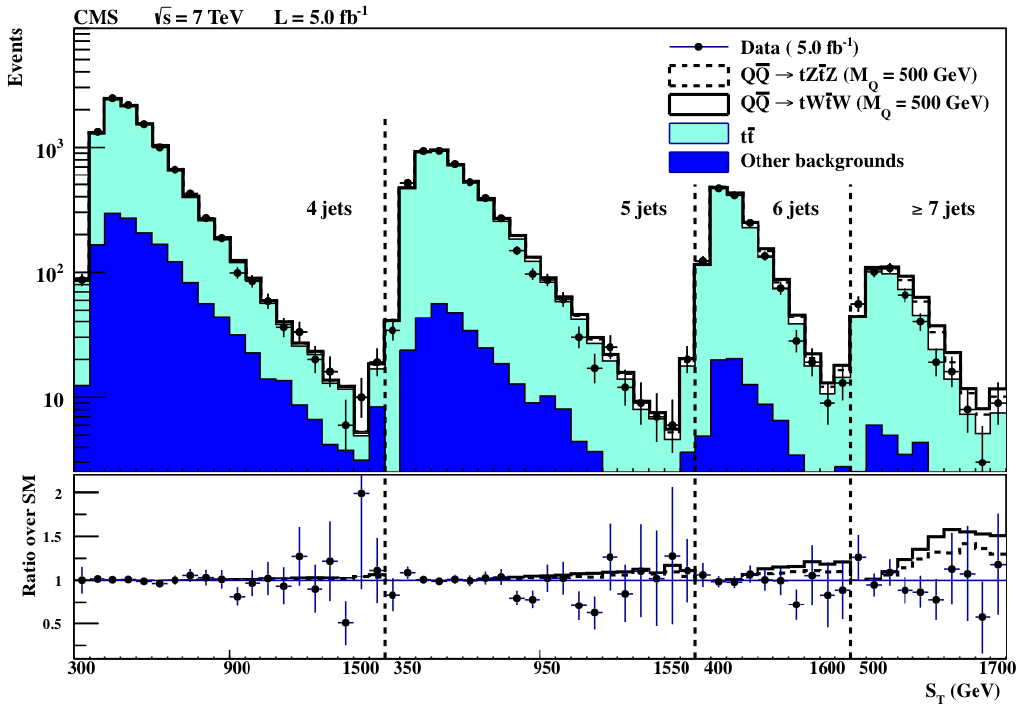
\includegraphics[width=0.6\linewidth]{physics_beyond_the_standard_model/lhc_4_gen_zoektocht.png}
    \caption{Zoektocht naar 4de generatie quarks in LHC}%
    \label{fig:physics_beyond_the_standard_model/lhc_4_gen_zoektocht}
\end{figure}

Uit de proton proton botsingen kunnen zowel 4, 5, 6 of 7 jets komen. Berekenen we alle mogelijke productie kanalen van deze jets zien we dat we bij de metingen niet echt afwijken van de voorspellingen. Er zit daar dus niet echt een 4de generatie aan quarks.

\subsection{Nieuwe uitwisseling bosonen}%
\label{sub:nieuwe_uitwisselings_bosonen}

Waarom zouden er geen extra $W'$ en $Z'$ bosonen bestaan. Misschien koppelen deze aan rechtshandige fermionen. Wie weet is $Z$ een samengestelde toestand en is daar een aangeslagen toestand van.

\begin{figure}[h]
    \centering
    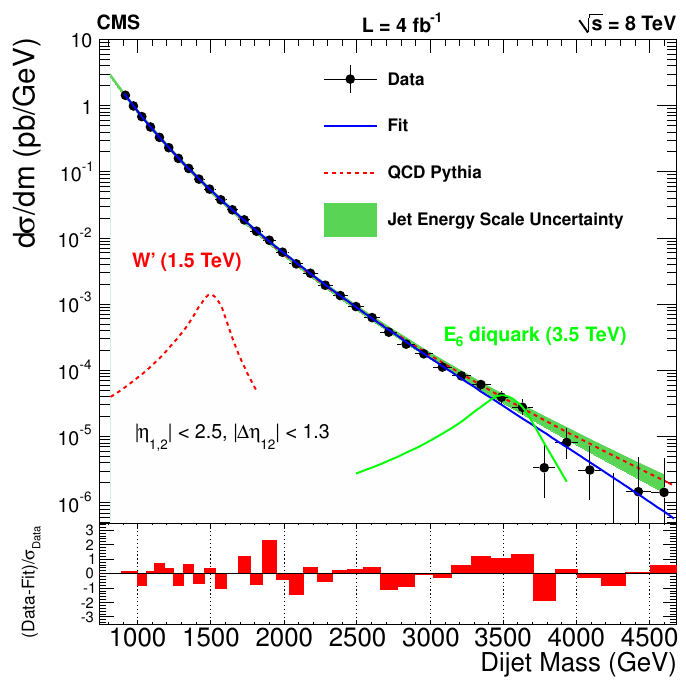
\includegraphics[width=0.4\linewidth]{physics_beyond_the_standard_model/cms_w'_z'_zoektocht.png}
    \caption{Zoektocht naar $W'$ en $Z'$ in LHC}%
    \label{fig:physics_beyond_the_standard_model/cms_w'_z'_zoektocht}
\end{figure}

We gaan kijken hier naar 2 jet fenomenen waar we hun gecombineerde massa uitzetten in vergelijking tot de werkzame doorsnede. De groene lijn is wat we verwachten en de blauwe lijn is wat we meten. We zien hier niet de spectra indien een $W'$ of diquark zou bestaan. Er is dus geen ruimte om af te wijken van het standaard model hier. Hetzelfde kunnen we vinden als we kijken naar de elektron positron vervallen. Er is hier ook geen plaats om de nieuwe intermediaire deeltjes toe te voegen aan het model.

\begin{figure}[h]
    \centering
    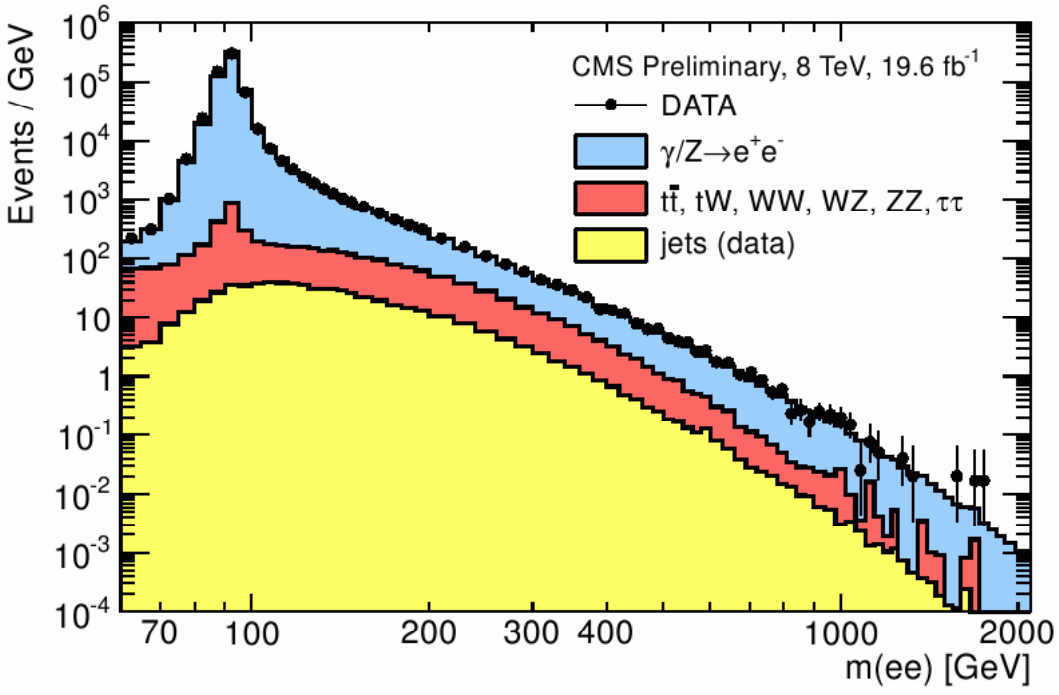
\includegraphics[width=0.6\linewidth]{physics_beyond_the_standard_model/ee_w'_z'_zoektocht.png}
    \caption{Zoektocht naar $W'$ en $Z'$ in LHC aan de hand van elektronen en positronen}%
    \label{fig:physics_beyond_the_standard_model/ee_w'_z'_zoektocht}
\end{figure}

\subsection{Zwarte gaten}%
\label{sub:zwarte_gaten}

Het is nu ook mogelijk om te zoeken naar zwarte gaten. Deze worden voorspelt door string theory. Deze voorspelt dat er nog veel meer dimensies zijn. In de opgerolde dimensies zou de zwaartekracht veel groter moeten zijn. Indien we deze dimensies zouden beginnen raken als we onze deeltjes maar dicht genoeg tot elkaar brengen zou het mogelijk moeten zijn om mini zwarte gaten te kunnen maken.
\begin{equation}
    \begin{aligned}
        \label{eq:zwarte_gaten}
        p p \rightarrow B H+X
    \end{aligned}
\end{equation}
Deze zijn heel klein en zouden zo goed als instant vervallen (verdampen) aan de hand van Hawking radiatie. Bij het maken van deze zwarte gaten zou een hoge multipliciteit aan finale toestanden moeten zijn van veel jets en leptonen. Om dit te onderzoeken kijken we of we zo evenementen kunnen vinden met grote jet aantallen.
\begin{figure}[h]
    \centering
    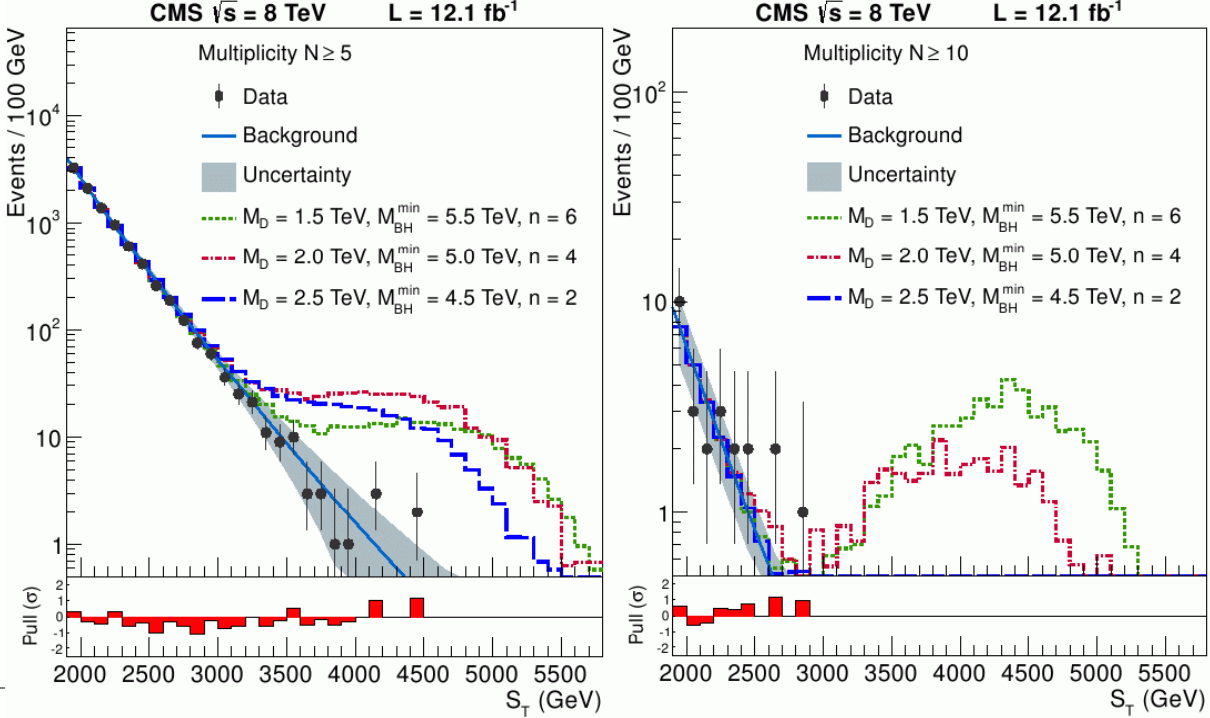
\includegraphics[width=0.6\linewidth]{physics_beyond_the_standard_model/zwarte_gaten.png}
    \caption{Zoektocht naar zwarte gaten}%
    \label{fig:physics_}
\end{figure}

In het blauw kan je de verwachtingen zien wat perfect zal kloppen met wat we zien. Indien we zwarte gaten zouden hebben met de massa's gegeven in de grafieken zouden we een grotere hoeveelheid aan evenementen verwachten bij grote $S_T$.

\subsection{Huidige toestand van direct onderzoek}%
\label{sub:huidige_toestand_van_direct_onderzoek}

Op dit moment hebben we nog niets gevonden maar kunnen mogelijke uitbreidingen van het standaard model uitsluiten tot op bepaalde hoeveelheden energie kunnen uitsluiten.

\begin{figure}[h]
    \centering
    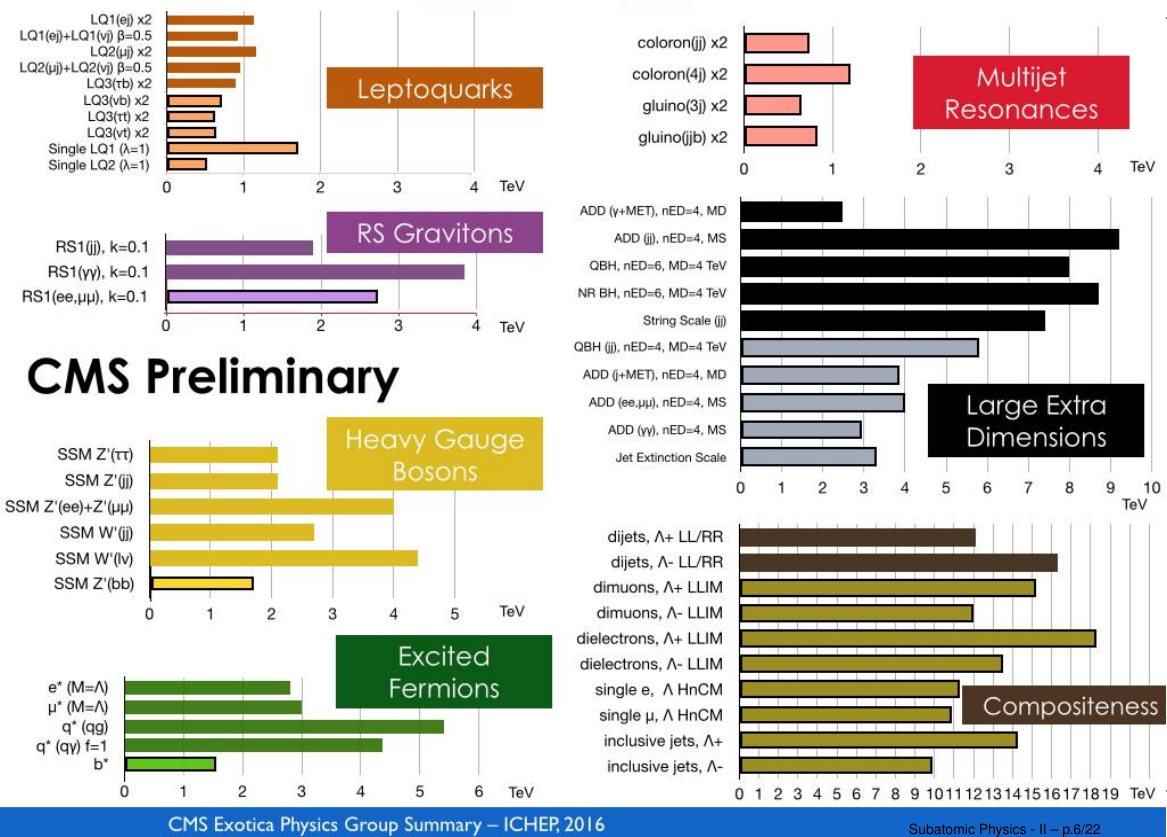
\includegraphics[width=0.6\linewidth]{physics_beyond_the_standard_model/current_state.png}
    \caption{Huidige toestand op deeltjes voorbij het Standaard Model}%
    \label{fig:physics_beyond_the_standard_model/current_state}
\end{figure}

Uiteindelijk is het een zoektocht naar hints die ons verder kunnen helpen in de zoektocht naar een meer complete theorie.

\subsection{Standaard Model}%
\label{sub:standaard_model}

Is het standaard model nu het ultieme model voor de wereld? Dat zou mogelijk kunnen zijn. Hierbij beschrijft de Dirac vergelijking de fermionen, QFT de interacties tussen de deeltjes. De interacties worden afgeleid uit een lokaal ijk principe. Het Higgs mechanisme om elektrozwakke symmetrie te breken en op die manier massa te creëren. Het ongemakkelijke in dit model is dat we al die parameters experimenteel moeten bepalen. Dit beschrijft alles wat we waarnemen, op enkele plaatsen zit daar spanning op maar hebben nog nooit een duidelijke afwijking gezien van het standaard model.\\
Al deze eigenschappen zijn er in gestoken. We weten hoe de Lagrangiaan er uit ziet maar niet waarom deze zo is. Wat we nu aan het onderzoeken zijn is waarom het Standaard model er zo uit ziet.\\
Wat zijn al deze vrije parameters nu in dit Standaard Model.
\begin{table}[h]
    \begin{minipage}[c]{0.48\textwidth}
        \centering
        \caption{Fermion sector}
        \label{tab:fermion_sector_parameters}
        \begin{tabular}{ccc}
            $m_{\nu_{1}}$   & $m_{\nu_{2}}$ & $m_{\nu_{3}}$ \\
            $m_{e}$         & $m_{\mu}$     & $m_{\tau}$ \\
            $m_{d}$         & $m_{s}$       & $m_{b}$ \\
            $m_{u}$         & $m_{c}$       & $m_{t}$
        \end{tabular}
        
        \caption{Ijk sector}
        \label{tab:ijk_sector}
        \begin{tabular}{ccc}
            $\alpha$ & $G_F$ & $\alpha_S$
        \end{tabular}
    \end{minipage}
    \begin{minipage}[c]{0.48\textwidth}
        \centering
        \caption{CKM, PMNS sector}
        \label{tab:ckm_pmns_sector}
        \begin{tabular}{cccc}
            $\lambda$       & $A$           & $\rho$        & $\eta$ \\
            $\theta_{12}$   & $\theta_{13}$ & $\theta_{23}$ & $\delta$
        \end{tabular}
        
        \caption{Higgs sector}
        \label{tab:higgs_sector}
        \begin{tabular}{cc}
            $v$ & $m_H$
        \end{tabular}

        \caption{QCD CP schending}
        \label{tab:qcd_cp_schending}
        \begin{tabular}{cc}
            $\theta_{CP}$
        \end{tabular}
    \end{minipage}
\end{table}

Indien er maar 1 van deze parameters er een beetje anders zou uit zien dan zou het heelal er totaal anders uit zien. De 26ste parameter, de $CP$ schending van de sterke wisselwerking is de enige die we nog niet hebben waargenomen. Indien er $CP$ schending voor de sterke wisselwerking zou zijn zouden we een dipoolmoment van het neutron waarnemen.

\subsection{Behouden grootheden}%
\label{sub:behouden_grootheden}

In de ruimte-tijd symmetrieën hebben we het behoud van energie, impuls, draaimoment en pariteit. We zijn vrij zeker dat deze allemaal behouden worden binnen de beperkingen van het heisenberg principe. Het behoud van lading, zwakke lading en kleur komen telkens overeen met een ijkveld, een veld symmetrie. Het Baryon getal $\mathcal{B}$ wordt blijkbaar behouden tot op zekere hoogte. Anders zou het universum vandaag de dag even veel baryonen als antibaryonen hebben. We zien dat het massa en het baryon getal verbonden zijn met elkaar door een massaloos veld dat eruit ziet als zwaartekracht. Er zit een kleine afwijking tussen het baryon getal en het massagetal vanwege de nucleaire binding. Het onderzoek naar dit massaloos veld is gedaan maar daar is niets gevonden. De koppeling van baryonen aan dit veld zou een stuk kleiner moeten zijn dan de koppeling van de zwaartekracht ($K<10^{-9}G$). Het is dus niet duidelijk waarom het baryon en lepton getal behouden worden in het Standaard Model.\\
Vandaag de dag zien we dat het de sterke interactie $CP$ niet zal schenden, $\theta_{C P} \approx 0$. Hier is geen a priori reden voor. Indien we zien dat iets behouden wordt, zijn we geneigd om daar een nieuw ijkveld aan te hangen, in dit geval een pseudoscalair veld. Indien er een nieuw ijkveld is, wordt er automatisch een nieuw ijkboson toegevoegd. In dit geval is de voorgestelde naam een axion wat een licht ($\sim 1\mu$eV-eV) neutraal pseudoscalair deeltje is. De eigenschappen van dit deeltje zijn slecht bepaald wat niet van belang is. Het moet er gewoon zijn en op een of andere manier koppelt aan de bestaande deeltjes. Dit geeft een lading en zou het $CP$ behoud verklaren. Dit zou dus opmengen met andere pseudoscalaire deeltjes zoals $\pi^0$ en $\eta$ die dan vervallen in 2 fotonen. Dit geeft een koppeling van axionen naar 2 fotonen. Het fuseren van 2 fotonen in een axion kan gebruikt worden om daar onderzoek naar te doen.

\begin{figure}[h]
    \centering
    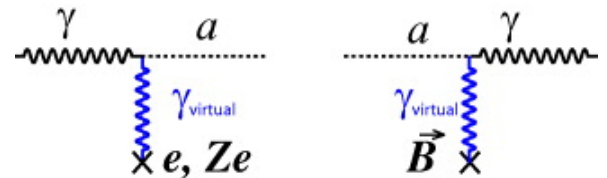
\includegraphics[width=0.4\linewidth]{physics_beyond_the_standard_model/axion_diagrammen.png}
    \caption{Feynman diagrammen waar we experimenteel naar op zoek zijn om het axion te vinden.}%
    \label{fig:physics_beyond_the_standard_model/axion_diagrammen}
\end{figure}

Hier annihileert een foton met een virtueel foton uit een magneetveld om een axion te maken dat dan terug in een magneetveld kan vervallen naar 2 fotonen. CAST doet dit onderzoek door fotonen in te laten invallen in een magneet van het LHC. Centraal staat een blok lood die de fotonen zal tegen houden maar niet de aangemaakte axionen die zo goed als niet interageren met materie. Deze axionen interageren achter het loodblok terug met het magneetveld en kijken dan of ze enige fotonen kunnen waarnemen.

\begin{figure}[h]
    \centering
    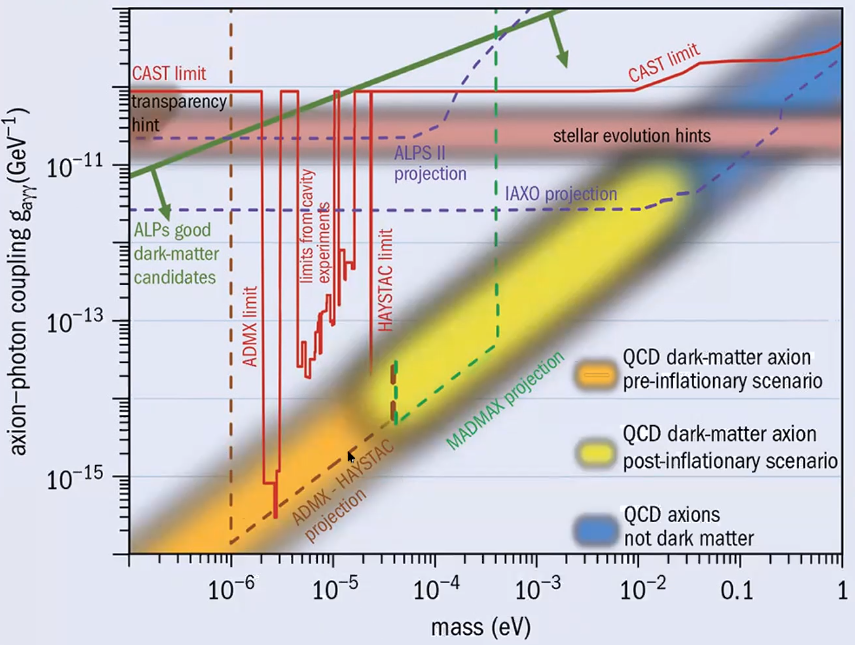
\includegraphics[width=0.6\linewidth]{physics_beyond_the_standard_model/cast_resultaten.png}
    \caption{Resultaten voor het onderzoek naar axionen}%
    \label{fig:physics_beyond_the_standard_model/cast_resultaten}
\end{figure}

Verticaal in de resultaten zichbaar in figuur \ref{fig:physics_beyond_the_standard_model/cast_resultaten} zie je de koppelingsterkte van axionen aan fotonen die niet a priori gegeven is en horizontaal de massa van de axionen. In de blauwe, gele en oranje band geven aan waar het axion zou moeten zitten als de juiste eigenschappen zou moeten hebben om het QCD $CP$ probleem op te lossen. Wat we uit de werking van sterren al kunnen zien is dat de fotonen niet al te sterk mogen koppelen aan de axionen omdat deze anders niet zouden werken zoals ze nu doen. De roze band geeft aan wat mogelijk zal zijn in functie van wat sterren doen. Indien de massa van de axionen iets hoger zou zijn dan is het mogelijk dat deze donkere materie zijn. Eén van de grootste redenen dat we denken dat er nog iets meer is dan het Standaard Model dat we nu kennen is het bestaan van donkere materie. We willen de link kunnen leggen tussen de subatomaire fysica en de astrofysica. Vandaag de dag met het Standaard Model beschrijven we maar 4 a 5\% van de massa van het heelal. Momenteel zijn we nog gelimiteerd in de limieten van onze metingen, we zijn nog niet mogelijk om preciezer te kijken dan de interstellaire limiet. Vandaag zien de uitgesloten gebieden er zo uit:

\begin{figure}[h]
    \centering
    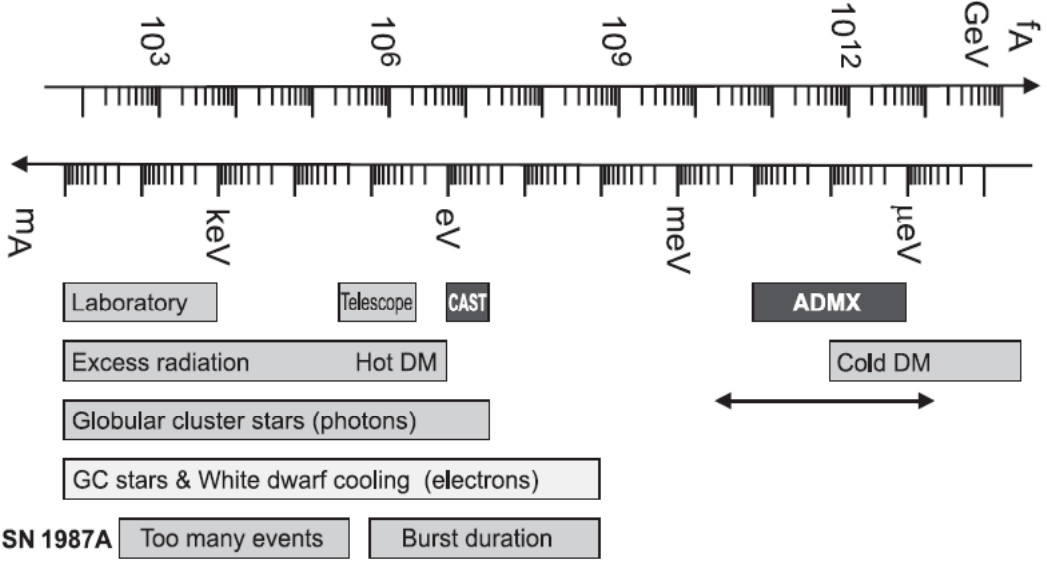
\includegraphics[width=0.6\linewidth]{physics_beyond_the_standard_model/axionen_verboden_gebieden.png}
    \caption{De verboden gebieden van de axionen}%
    \label{fig:physics_beyond_the_standard_model/axionen_verboden_gebieden}
\end{figure}

\subsection{Grand Unified Theories}%
\label{sub:grand_unified_theories}

Voor het uitwisselen van kleine hoeveelheden energie zien we dat de koppelingconstantes van de sterke, zwakke en elektromgnetische wisselwerking grote verschillen tonen. We hebben ook gezien dat dit lopende koppelingconstantes zijn. Voor grotere en grotere hoeveelheden aan energie lijken deze naar elkaar toe te gaan. Extrapoleren we wat we vandaag de dag kennen, dan verwachten we bij het uitwisselen van $q=M_{X} \sim 10^{15}$ de krachten even sterk zouden moeten zijn.

\begin{figure}[h]
    \centering
    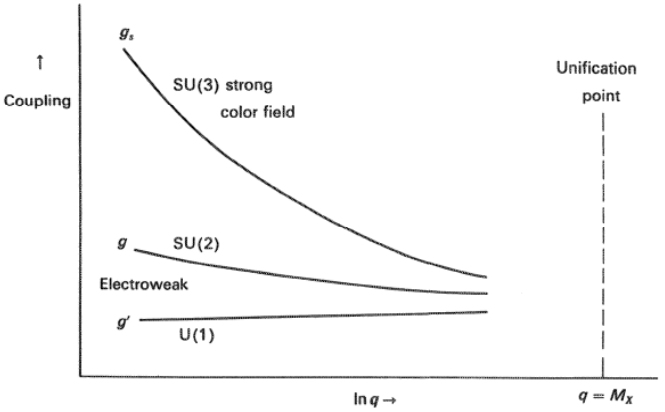
\includegraphics[width=0.5\linewidth]{physics_beyond_the_standard_model/grand_unified_theory.png}
    \caption{Lopende koppelingconstantes in de Grand Unified Theory}%
    \label{fig:physics_beyond_the_standard_model/grand_unified_theory}
\end{figure}

In 1974 waren de eerste ideeën er al om deze krachten te unificeren. Hier zouden ze $SU(1)$, $SU(2)$ en $SU(3)$ samen te brengen tot 1 grotere ijk symmetrie $SU(5)$. Deze $SU(5)$ groep zou zo goed als automatisch uiteen vallen in de 3 groepen die we nu al hebben. Deze theorie zo 24 ijkbosonen bevatten. Deze zijn
\begin{itemize}
    \item 8 gluonen
    \item 3 zwakke bosonen, de $W$ en $Z$ bosonen
    \item het foton
    \item 12 nieuwe ijkbosonen $Y$ en $X$ de leptoquarks
\end{itemize}
Zoals de elektrozwakke symmetrie die wordt gebroken door het Higgs boson zal de Grand Unified Theory symmetrie ook gebroken worden. Deze breuk zou moeten leven bij ongeveer $m_{Y} \sim m_{X} \sim 10^{15}$GeV (Zelf bij kosmische straling fysica komen we maar aan $10^{12}$GeV.). Naast de massa van de $Y$ en $X$ bosonen moeten er ook GUT-Higgs bosonen zijn. Uit de theorie zijn de massa van de bosonen gegeven door: $Q_{Y}=-\frac{1}{3}$ en $Q_{X}=-\frac{4}{3}$. Ze hebben naar een lading ook 3 mogelijke kleuren wat in het totaal 12 verschillende mogelijkheden moet geven. Omdat ze een massa hebben zouden deze moeten vervallen in onze deeltjes die we al kennen. Een aantal voorbeelden van zo een vervallen zijn: $X_{1} \rightarrow e^{-} d, \bar{u} \bar{u}$ en $Y_{2} \rightarrow \mu^{-} c, \bar{c} \bar{s}$. De multipletten die we bij deze theorie nu krijgen zijn vrij verschillend, we krijgen hier quintetten en decupletten.
\begin{equation}
    \begin{aligned}
        \label{eq:qut_multipletten}
        \overline{5}&=\left(\begin{array}{c}
                \nu_{e} \\
                e^{-} \\
                \bar{d}_{R} \\
                \bar{d}_{B} \\
                \bar{d}_{G}
        \end{array}\right)_{L H}\\
        10&=\left(\begin{array}{ccccc}
                0 & e^{+} & d_{R} & d_{B} & d_{G} \\
                -e^{+} & 0 & u_{R} & u_{B} & u_{G} \\
                -d_{R} & -u_{R} & 0 & \bar{u}_{G} & \bar{u}_{B} \\
                -d_{B} & -u_{B} & -\bar{u}_{G} & 0 & \bar{u}_{R} \\
                -d_{G} & -u_{G} & -\bar{u}_{B} & -\bar{u}_{R} & 0
        \end{array}\right)_{L H}
    \end{aligned}
\end{equation}
Wat we zien gebeuren is dat de som van de ladingen in de multipletten 0 zal moeten zijn, $\sum_{i} Q_{i}=0$. Dit verklaard waarom we de $-1/3$ en $2/3$ lading hebben voor onze quarks en de gelijkheid $Q(\nu)-Q(e)=Q(u)-Q(d)$.\\
\begin{center}
    \feynmandiagram [layered layout, horizontal=b to c] {
        a [particle=\(Z^0\)] -- [photon] b
        -- [fermion, half left, looseness=1.5] c
        -- [fermion, half left, looseness=1.5] b,
        c -- [photon] d [particle=\(\gamma\)],
    };
\end{center}
Technisch gezien is het feynman diagram hierboven waar te nemen. Voor het Standaard Model weten we uit de elektrozwakke theorie dat die orthogonaal moeten staan op elkaar bij constructie $\left< Z^0\mid \gamma\right> = 1$. Bij de berekening van het matrix element via de Grand Unified Theory zien we iets anders tevoorschijn komen.
\begin{table}[h]
    \centering
    \begin{tabular}{c|cc}
        & $I_{3}$ & $Q$ \\
        \hline
        $\left(\nu_{e}\right)_{L H}$ & $+1 / 2$ & $0$ \\
        $\left(e^{-}\right)_{L H}$ & $-1 / 2$ & $-1$ \\
        $\left(\bar{d}_{R}\right)_{L H}$ & $0$ & $+1 / 3$ \\
        $\left(\bar{d}_{B}\right)_{L H}$ & $0$ & $+1 / 3$ \\
        $\left(\bar{d}_{G}\right)_{L H}$ & $0$ & $+1 / 3$
    \end{tabular}
\end{table}
\begin{equation}
    \begin{aligned}
        \label{eq:z_to_gamma_gut}
        \sum Q\left(I_{3}-Q \sin ^{2} \theta_{W}\right) &=0 \\
        \Rightarrow \sin ^{2} \theta_{W}\left(M_{X}^{2}\right)=\frac{\sum Q I_{3}}{\sum Q^{2}} &=\frac{3}{8}
    \end{aligned}
\end{equation}
Zo is het mogelijk om $\sin^2\theta_W$ te bepalen bij de GUT schaal. Evolueren we dit terug naar de schaal waar we de massa van het $Z$ boson kennen aan de hand van $g^{\prime} / g=\tan \theta_{W}$ en vinden we $\sin ^{2} \theta_{W}\left(M_{Z}^{2}\right) \approx 0.21$ wat dicht bij de waarde ligt die we vandaag de dag kennen van $0.23$ maar dit is nog buiten de fout. Eén groot probleem dat we nu zien is dat het proton kan vervallen $p \rightarrow e^{+} \pi^{0}$.

\begin{figure}[h]
    \centering
    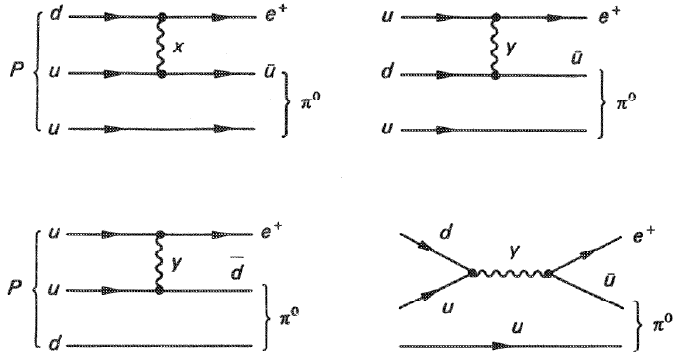
\includegraphics[width=0.6\linewidth]{physics_beyond_the_standard_model/proton_verval.png}
    \caption{Feynman diagrammen van het proton verval}%
    \label{fig:physics_beyond_the_standard_model/proton_verval}
\end{figure}

Ten eerste hebben we hier geen behoud van het baryon getal en lepton getal. We zijn dus duidelijk voorbij het Standaard Model. Deze vervallen zullen vooral gedomineerd worden door hoe waarschijnlijk het is dat een deeltje met massa $M_X$ aangemaakt wordt. Het dominante deel in de propagator is $\frac{1}{q^{2}+M_{X}^{2}}$. Wat de levensduur betreft zal deze de inclusie van deze massa tot de 4de macht heel groot zijn $\tau \approx \frac{1}{\alpha^{2}} \frac{M_{X}^{4}}{M_{p}^{5}} \sim 10^{31} \text { yr }$. Experimenteel is dit sinds het begin van het inversum nog nooit waargenomen en hebben we $\tau\left(p \rightarrow e^{+} \pi^{0}\right) \geq 8.4 \times 10^{33} \text{yr}$. Dit onderzoek was initieel gedaan aan Kamiokande waar ze gewoon kijken naar een grote hoeveelheid water waar er mogelijks opeens een proton zou vervallen.\\
Uit al deze problemen zijn we zeker dat de $SU(5)$ implementatie van de GUT zeker niet de oplossing zal zijn. Maar dit wil niet zeggen dat we er niet dicht bij komen. Er zijn hier al veel correcte elementen aanwezig. We gaan dus zoeken of een complexer alternatief wel het goede antwoord zou geven. Het probleem hierbij is dat deze steeds meer ijkbosonen geven die we niet hebben waargenomen. Het onderzoek naar leptoquarks wordt natuurlijk ook gedaan bij HERA ($e+q \rightarrow X / Y \rightarrow q q$) waar we nog niets hebben gevonden. Dit geeft aanleiding dat er niets zou zijn tussen $M_{EW}$ en $M_{GUT}$. Dit omdat als we ze zouden bestaan maar nog niet aan hun massa komen, zouden we er toch al gevoelig voor moeten zijn. Denk aan de lus diagrammen die kunnen optreden in vorige hoofdstukken.

\subsection{Compositen}%
\label{sub:compositen}

Een concept dat in het verleden al heel succesvol is geweest, is veronderstellen dat de deeltjes die we nu kennen bestaan uit sub-deeltjes gebonden door een heel sterke interactie. Deze deeltjes noemen we preonen. Een voorbeeld van zo een theorie is de Rishon-theorie. Deze introduceert 2 nieuwe deeltjes $T$ en $V$ met als ladingen $Q_{T}=+1 / 3$ en $Q_{V}=0$. Deze kunnen we gebruiken om de gekende deeltjes te beschrijven:
\begin{equation}
    \begin{aligned}
        \label{eq:rischon_samenstelling}
        \left| e^{+}\right>&=\left| T T T\right>\\
        \left| \nu_{e}\right>&=\left| V V V\right>\\
        \left|u\right> &=\left|T T V\right>,\left| T V T\right>, \left| V T T\right>\text { for } 3 \text { colours } \\
        \left| \bar{d}\right>&=\left|T V V\right>\left| V T V\right>, \left| V V T\right>\text { for } 3 \text { colours } \\
        \left|W^{+}\right\rangle &=\left| T T T V V V\right>
    \end{aligned}
\end{equation}
Er is hier 1 fundamenteel probleem. Uit de diep inelastische verstrooiing hebben we voor de afmeting voor het elektron en het quark ten hoogste $10^{-18}$m zijn. Als we die deeltjes op zo een kleine plaats willen opsluiten weten we door het heisenberg principe dat de impuls van $T$ en $V$ rond de 200GeV zal moeten zitten. Om die 600GeV aan energie te reduceren naar enkele $m_f\sim$MeV moeten we bindings energie van de orde een $O(100s)$GeV hebben. Het groot zijn en elkaar juist uit cancellen om die enkele MeV te bekomen zit niet goed. Dit is de reden waarom we denken dat we aan de effectieve bouwstenen zitten van het universum met de elementaire deeltjes.\\
We zouden ook nog verwachten dat onze elementaire deeltjes aangeslagen toestanden hebben. Hierbij zouden de verschillende generaties overeen komen met een hyperfijn structuur. Indien dit zo is zouden we deze moeten zien vervallen $f^{*} \rightarrow f \gamma$ en $q^{*} \rightarrow q g, q \gamma$ wat we ook nog niet hebben gevonden.

\subsection{Supersymmetrie}%
\label{sub:supersymmetrie}

Indien we geloven dat GUT bestaat komt er 1 groot probleem naar boven, dit noemen we het hiërarchie probleem. Bij deze schalen van $\Lambda_{G U T} \sim 10^{16}$GeV of $\Lambda_{P} \sim 10^{19}$GeV zal het Higgs boson naast de typische loop diagrammen op de eerste rij zullen de loop diagrammen ook gebeuren met het $X$ boson.

\begin{figure}[h]
    \centering
    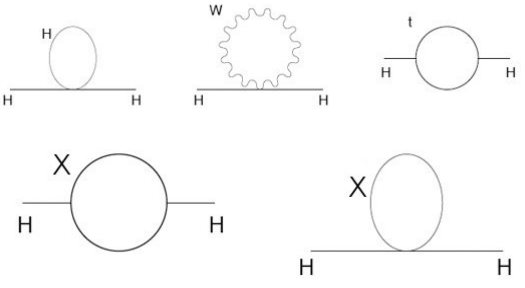
\includegraphics[width=0.5\linewidth]{physics_beyond_the_standard_model/loop_diagrammen_higgs.png}
    \caption{Loop diagrammen van het Higgs bij GUT en planck schaal}%
    \label{fig:physics_beyond_the_standard_model/loop_diagrammen_higgs}
\end{figure}

Zoals eerder in kwantumvelden is aangetoond is de massa van het Higgs boson zijn naakte massa plus al de loop diagrammen die we hier hebben.
\begin{equation}
    \begin{aligned}
        \label{eq:massa_higgs}
        M_{H}^{2}=M_{0}^{2}+\sum_{i} c_{i} \Lambda^{2}
    \end{aligned}
\end{equation}
De toevoeging van de loopdiagrammen aan $X$ zullen een gigantische hoeveelheid extra massa geven aan het Higgs boson. Als er iets is voorbij het Standaard Model, en dat moet er bijna zijn, zal bij deze schalen de zelfkoppeling van die deeltjes de massa van het Higgs boson flink opdrijven. Het probleem is dat ons Higgs deeltje licht is, om goed te zijn zou het veel zwaarder moeten zijn. De diagrammen die we nu hebben toegevoegd zouden dus moeten gecompenseerd worden met nog andere diagrammen.

\begin{figure}[h]
    \centering
    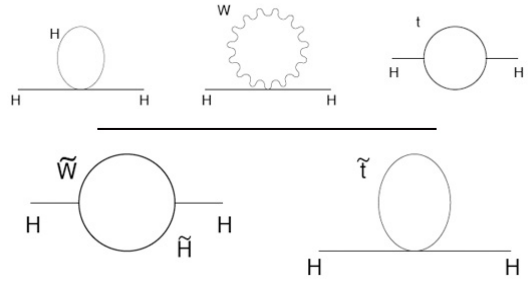
\includegraphics[width=0.5\linewidth]{physics_beyond_the_standard_model/sussy_deeltjes.png}
    \caption{Invoeren van equivalenten aan het $W$ boson en $t$ quark interacties}%
    \label{fig:physics_beyond_the_standard_model/sussy_deeltjes}
\end{figure}

Hoe kunnen we die cancelaties nu implementeren? Introduceren we nieuwe deeltjes die koppelen aan het Higgs. Voor elke koppeling van het Higgs aan het $W$ deeltje krijgen we een koppeling aan het $\tilde{W}$ deeltje en hetzelfde voor de $t$ quark en alle andere koppelingen. Door de koppeling van $W$ te linken aan de koppeling van $\tilde{W}$ aan het Higgs is de cancelatie is ingebouwd in de theorie. Indien de overeenkomstige deeltjes zelf perfect hetzelfde zijn, cancelt alles elkaar uit en heeft het Higgs een massa van 0. Het invoeren van dit concept is de supersymmetrie (=SUSY). Dit zou al moeten werken voor SUSY deeltje met $M_{SUSY}<1$TeV. In het LHC hadden we verwacht dat het Higgs boson moeilijk te vinden zou geweest zijn maar dat we ook SUSY deeltjes zouden gevonden hebben.\\
Hoe zien de SUSY deeltjes er nu uit? Om dit te bekijken vergelijken we de krachten van de van de $SU(5)$ theorie en de supersymmetrie.

\begin{figure}[h]
    \centering
    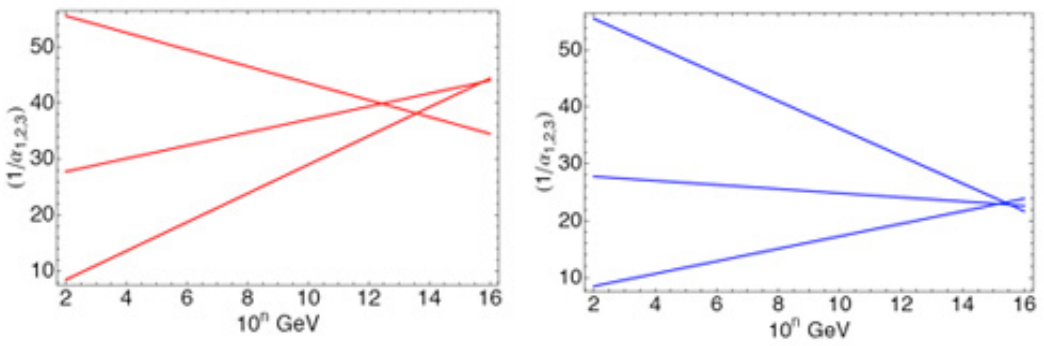
\includegraphics[width=0.5\linewidth]{physics_beyond_the_standard_model/su5_vs_susy.png}
    \caption{Vergelijking van de krachten in $SU(5)$ en SUSY}%
    \label{fig:physics_beyond_the_standard_model/su5_vs_susy}
\end{figure}

Je ziet direct dat de krachten voor de $SU(5)$ theorie niet zullen convergeren tot 1 punt, de SUSY krachten doen dit wel bij $\sim 10^{-16}$GeV. Dit komt door de extra ingebouwde vrijheidsgraad, de massa schaal van die deeltjes. Daar kan je dus mee spelen. De voorwaarde is dat de SUSY deeltje van de orde $\Lambda \sim 1$TeV zijn. Op deze manier hebben we een symmetrie toegevoegd tussen de bosonen en fermionen. Deze symmetrie zien we op dit moment niet. Op dit moment zien we een asymmetrie tussen de fermionen die materie deeltjes zijn en bosonen wat krachtdeeltjes zijn. Het is de supersymmetrie die gebroken wordt die voor de elektrozwakke breking $\sim 100$GeV is en voor SUSY ongeveer 1TeV.\\
SUSY is de laatste symmetrie tussen de fermionen en bosonen. Voor elk boson voegen we een fermion toe en voor elk fermion een boson. We hebben nu dus dubbel zo veel deeltjes. Nemen we als voorbeeld het spin 1/2 quark $u$.
\begin{equation}
    \begin{aligned}
        \label{eq:susy_deeltjes_1}
        \begin{array}{llllll}
            \text{ spin } \frac{1}{2} & u: \text{u}_{L} & u_{R} & \bar{u}_{L} & \bar{u}_{R} & (3 \text { colours }) \Rightarrow 12 \text { d.o.f. } \\
            \text { spin } 0 & \tilde{u}: \widetilde{u_{L}} & \widetilde{u_{R}} & \widetilde{\bar{u}_{L}} & \widetilde{\bar{u}_{R}} & (3 \text { colours }) \Rightarrow 12 \text { d.o.f. }
        \end{array}
    \end{aligned}
\end{equation}
De SUSY equivalenten van de up quark noemen we de s(up)quark. Belangrijk is dat $\widetilde{u_{L}}$ geen links handig deeltje is, deze heeft geen spin en dus geen handigheid. Zo hebben we ook de sneutrinos, de gluinos (zou 3 spin vrijgheidsgraden moeten hebben maar door massaloos te zijn is er 1 weg gevallen)
\begin{equation}
    \begin{aligned}
        \label{eq:susy_deeltjes_2}
        \begin{array}{llll}
            \text{ spin } \frac{1}{2} & \nu: \nu_{L} & \bar{\nu}_{R} & \Rightarrow 2 \text { d.o.f. } \\
            \text{ spin } 0 & \tilde{\nu}: \widetilde{\nu_{L}} & \widetilde{\nu_{R}} & \Rightarrow 2 \text { d.o.f. }
        \end{array}\\
        \begin{array}{lll}
            \text { spin } 1 & g & 2 \text{ spin } \times 8 \text { colour } \Rightarrow 16 \text { d.o.f. } \\
            \text{ spin } \frac{1}{2} & \tilde{g} & 2 \text{ spin } \times 8 \text { colour } \Rightarrow 16 \text { d.o.f. }
        \end{array}
    \end{aligned}
\end{equation}
In het Standaard model hebben we:
\begin{itemize}
    \item in de elektrozwakke sector
        \begin{equation}
            \begin{aligned}
                \label{eq:susy_deeltjes_3}
                \begin{array}{lcccccc} 
                                        & B & W^{0} & W^{1} & W^{2} & \Phi  & \\
                    \text { d.o.f. }    & 2 & 2     & 2     & 2     & 4     & \sum=12
                \end{array}
            \end{aligned}
        \end{equation}
    \item achter de EW-symmetrie breking
        \begin{equation}
            \begin{aligned}
                \label{eq:susy_deeltjes_4}
                \begin{array}{lcccccc} 
                                        & \gamma & Z^{0} & W^{+} & W^{-} & H  & \\
                    \text { d.o.f. }    & 2 & 3     & 3     & 3     & 1     & \sum=12
                \end{array}
            \end{aligned}
        \end{equation}
\end{itemize}
Schakelen we over naar SUSY dan hebben we 2 scalaire velden nodig hebben (Hebben 4 extra higgs velden nodig) krijgen we:
\begin{itemize}
    \item in de elektrozwakke sector in SUSY
        \begin{equation}
            \begin{aligned}
                \label{eq:susy_deeltjes_5}
                \begin{array}{llcccccc} 
                    & B & W^{0} & W^{1} & W^{2} & \Phi_{u} & \Phi_{d} & \\
                    \text { d.o.f. } & 2 & 2 & 2 & 2 & 4 & 4 & \sum=16
                \end{array}
            \end{aligned}
        \end{equation}
    \item achter de EW-symmetrie breking
        \begin{equation}
            \begin{aligned}
                \label{eq:susy_deeltjes_6}
                \begin{array}{lllclllllll} 
                    & \gamma & Z^{0} & W^{+} & W^{-} & h & H & A & H^{+} & H^{-} & \\
                    \text {d.o.f. } & 2 & 3 & 3 & 3 & 1 & 1 & 1 & 1 & 1 & \sum=16
                \end{array}
            \end{aligned}
        \end{equation}
        Al deze extra Higgs bosonen zijn nog steeds scalair maar kunnen nu ook een lading hebben.
    \item Hun SUSY equivalenten zijn
        \begin{equation}
            \begin{aligned}
                \label{eq:susy_deeltjes_7}
                \begin{array}{lccccccccc} 
                    & \tilde{\chi}_{1}^{0} & \tilde{\chi}_{2}^{0} & \tilde{\chi}_{3}^{0} & \tilde{\chi}_{4}^{0} & \tilde{\chi}_{1}^{+} & \tilde{\chi}_{1}^{-} & \tilde{\chi}_{2}^{+} & \tilde{\chi}_{2}^{-} & \\
                    \text {d.o.f. } & 2 & 2 & 2 & 2 & 2 & 2 & 2 & 2 & \sum=16
                \end{array}
            \end{aligned}
        \end{equation}
        Dit zijn allemaal spin $1/2$ deeltjes.
\end{itemize}
De leuke van al deze deeltjes zijn de neutralinos $\tilde{\chi}^{0}$ en de charginos $\tilde{\chi}^{\pm}$. Naast het invoeren van de symmetrie en de deeltjes zal er ook een nieuwe pariteit tevoorschijn komen, de $R$-pariteit. Deze pariteit maakt het onderscheid tussen deeltjes en s-deeltjes.
\begin{equation}
    \begin{aligned}
        \label{eq:r_pariteit}
        R=(-1)^{2 S+3(\mathcal{B}-\mathcal{L})}
    \end{aligned}
\end{equation}
Hier komen de baryon en lepton getallen in voor wat van groot belang is. Indien $R$ is behouden moet zijn volgen daar een aantal dingen uit.
\begin{itemize}
    \item Als je een s-deeltje maakt moet je ook zijn s-antideeltje maken, ze worden aangemaakt in paren.
    \item De lichtste s-deeltje moet stabiel zijn (LSP). In de meeste modellen is dit het neutralino $\tilde{\chi}_{1}^{0}$. Omdat hij ongeladen is zal hij enkel interageren met de zwakke interactie. Net zoals de neutrinos ontsnappen deze gewoon uit de detector en zien we dit als $E_{\text {mis }}$ en $\vec{p}_{\text {mis }}$. Het neutralino heeft een massa van ongeveer $100$GeV en dus een perfecte kandidaat voor de donkere materie.
    \item Het baryon en lepton getal zullen niet behouden worden maar de combinatie $\mathcal{B}-\mathcal{L}$ wel.
\end{itemize}
Nu kunnen we beginnen zoeken naar deze deeltjes. Indien SUSY exact zou zijn hebben we $m_{P}=m_{\tilde{P}}$. Dit is overduidelijk niet zo want een up s-quark zou dezelfde massa moeten hebben als een up quark. De SUSY moet dus gebroken worden. Dit kan mogelijks gebeuren aan de hand van spontane symmetrie breking aan de GUT-schaal of via gravitatie bemiddelde breking (wat super symmetric gravity is SUGRA). Om de massa van het Higgs boson stabiel te moeten krijgen moet de massa schaal van de orde 1TeV zijn.\\
Er zijn veel verschillende modellen voor SUSY waarvan sommige $R$ niet behouden is maar wat ze allemaal gemeen hebben is dat er gigantisch veel nieuwe parameters worden toegevoegd. De zoektocht naar de correcte supersymmetrie theorie zal dus heel complex zijn.

\subsection{Zoektocht naar SUSY}%
\label{sub:zoektocht_naar_susy}

We overlopen hier een aantal mogelijke scenarios hoe we er achter SUSY kunnen zoeken. Ten eerste kunnen we zoeken naar s-lepton productie.
\begin{equation}
    \begin{aligned}
        \label{eq:slepton_productie}
        l+\bar{l} \rightarrow Z^{*} \rightarrow \tilde{l}+\tilde{\bar{l}}
    \end{aligned}
\end{equation}
Maken we op deze manier bijvoorbeeld s-muonen die vervallen naar $\tilde{\mu} \rightarrow \mu+\tilde{\chi}_{1}^{\theta}$. Indien $m_{\tilde{\mu}}>m_{\tilde{\chi}_{1}^{0}}$ is zal dit proces mogelijks een $\mu^\pm$ paar kunnen aanmaken. Indien $\Delta m=m_{\tilde{\mu}}-m_{\tilde{\chi}_{1}^{0}}$ groot genoeg is zouden we het paar kunnen waarnemen. Indien we het observeren moeten we het paar waarnemen en een tekort aan energie. Dit hebben we niet gevonden.\\
Een ander scenario is zoeken naar s-quarks en gluinos. Deze aan de hand van de sterke interactie gemaakt in plaats van de zwakke. Dit moet dus gebeuren aan hadron colliders, we zouden er veel meer moeten kunnen maken. Indien $m_{\tilde{q}} \ll m_{\tilde{g}}$ dan domineert de $\tilde{q} \tilde{\bar{q}}, \tilde{q} \tilde{q}$ productie. De (anti)s-quarks vervallen tot (anti)quarks $\tilde{q} \rightarrow q \tilde{\chi}_{1}^{0}$. In deze processen zien we dus 2 jets met een missende hoeveelheid energie. Een belangrijke opmerking hier is dat we de s-quarks aanmaken met de sterke interactie en vervallen aan de hand van de SUSY reactie wat ons doet herinneren aan de kaonen die zullen opmengen. Indien $m_{\tilde{g}} \ll m_{\tilde{q}}$ is domineert de $\tilde{g} \tilde{g}$ productie. Deze gluinos vervallen als volgt: $\tilde{g} \rightarrow \tilde{q} \bar{q} \rightarrow q \bar{q} \tilde{\chi}_{1}^{0}$. Zo nemen we 4 jets met een deel missende energie waar.\\
Hetzelfde voor charginos en neutralinos:
\begin{equation}
    \begin{aligned}
        \label{eq:char_neutr_prod}
        p+p & \rightarrow \tilde{\chi}_{1}^{\pm}+\tilde{\chi}_{2}^{0} \\
        \tilde{\chi}_{2}^{0} & \rightarrow Z^{*}+\tilde{\chi}_{1}^{0} \rightarrow l^{+} l^{-}+\tilde{\chi}_{1}^{0} \\
        \tilde{\chi}_{1}^{\pm} & \rightarrow W^{\pm}+\tilde{\chi}_{1}^{0} \rightarrow l^{\pm} \nu_{l}+\tilde{\chi}_{1}^{0}
    \end{aligned}
\end{equation}
Hier neem je 3 leptonen en een deel missende energie waar.

\begin{figure}[ht]
    \centering
    \subfloat[stop productie]{
        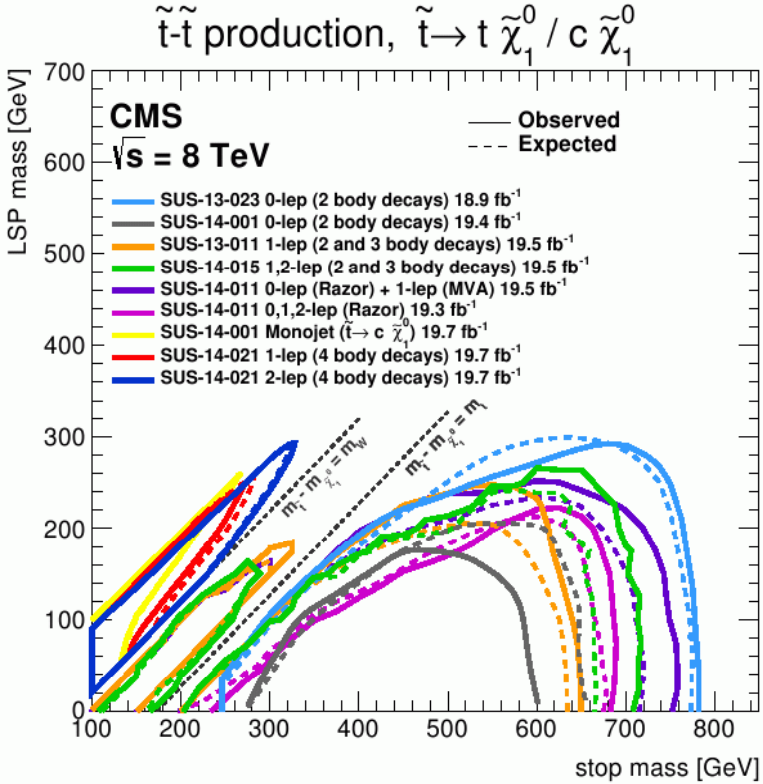
\includegraphics[width=0.3\textwidth]{physics_beyond_the_standard_model/stop_productie.png}
    }
    \hfill
    \subfloat[gluino productie]{
        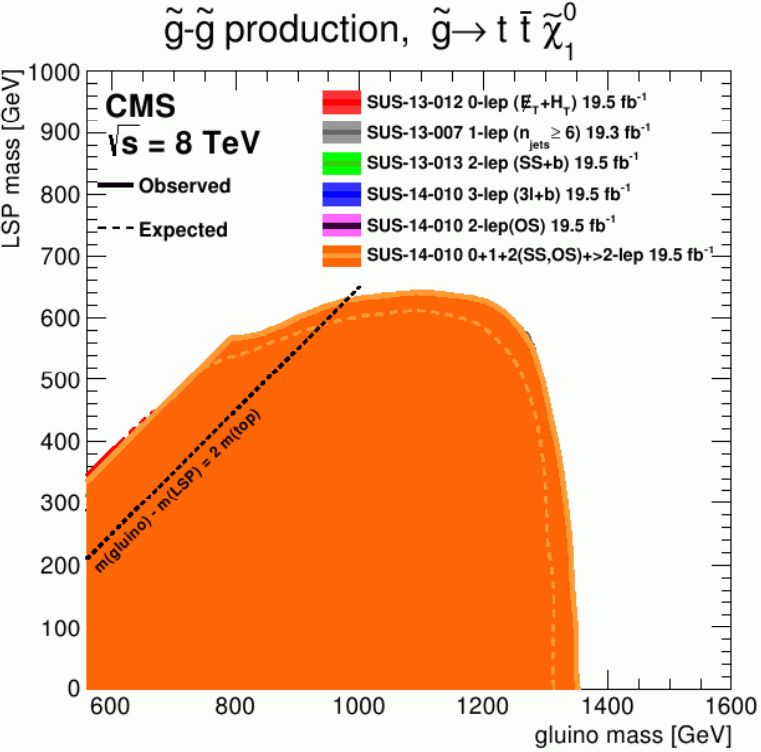
\includegraphics[width=0.3\textwidth]{physics_beyond_the_standard_model/gluino_productie.png}
    }
    \hfill
    \subfloat[chargino en neutralino productie]{
        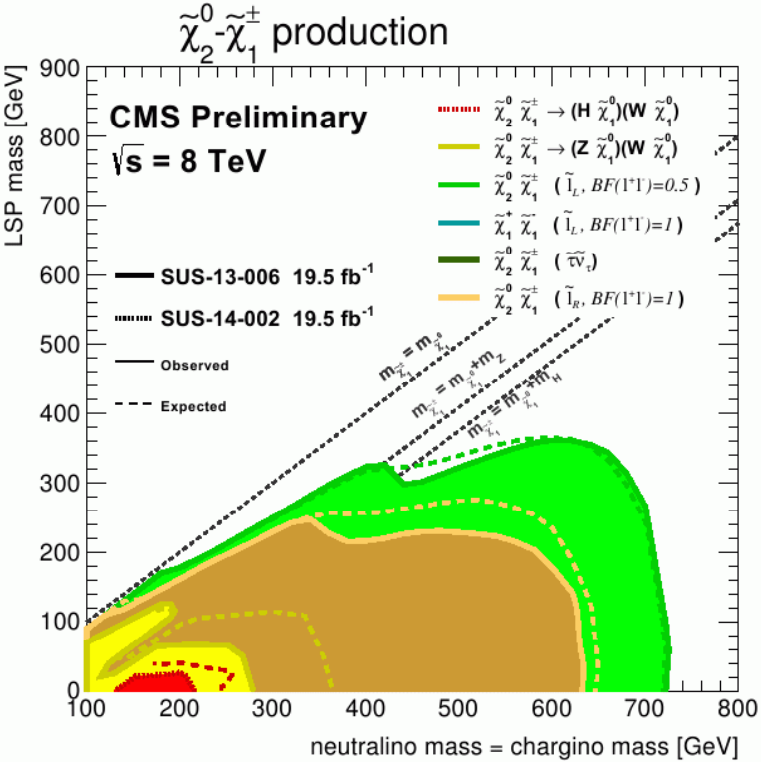
\includegraphics[width=0.3\textwidth]{physics_beyond_the_standard_model/chargino_neutralino_productie.png}
    }\\
    \subfloat[SUSY zoektocht anno 2013]{
        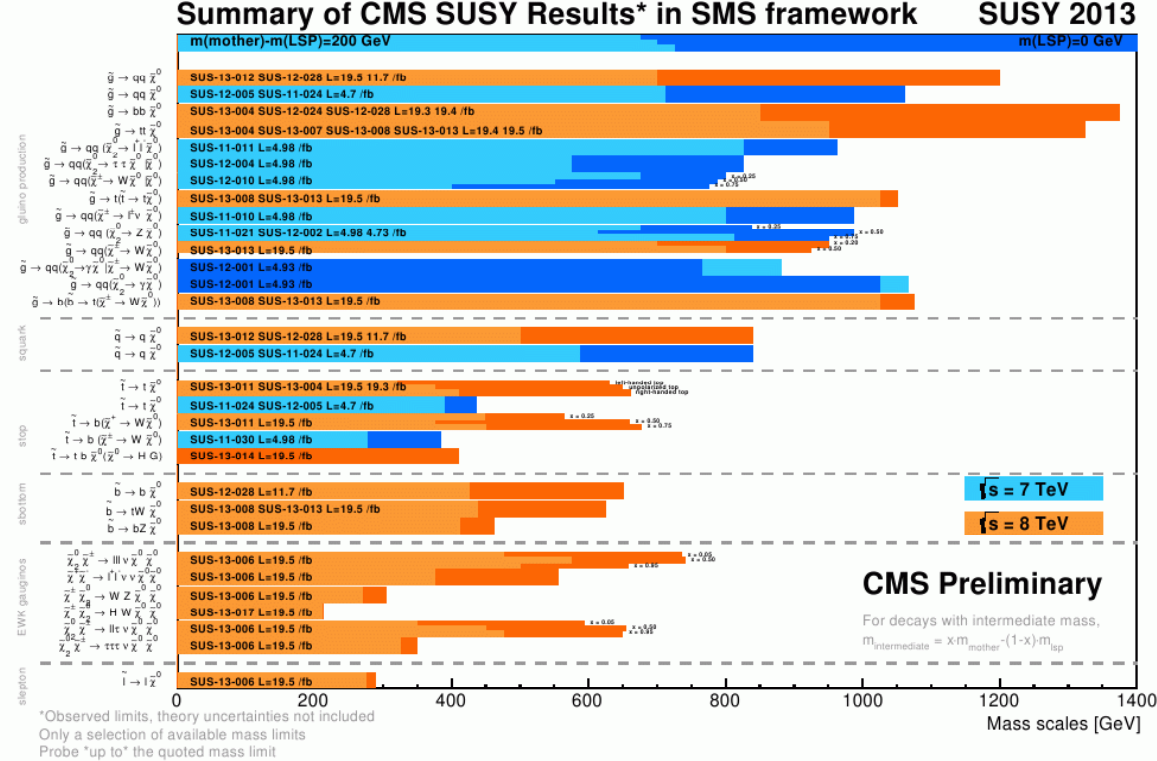
\includegraphics[width=0.4\textwidth]{physics_beyond_the_standard_model/susy_zoektocht_2013.png}
    }
    \hfill
    \subfloat[SUSY zoektocht anno 2017]{
        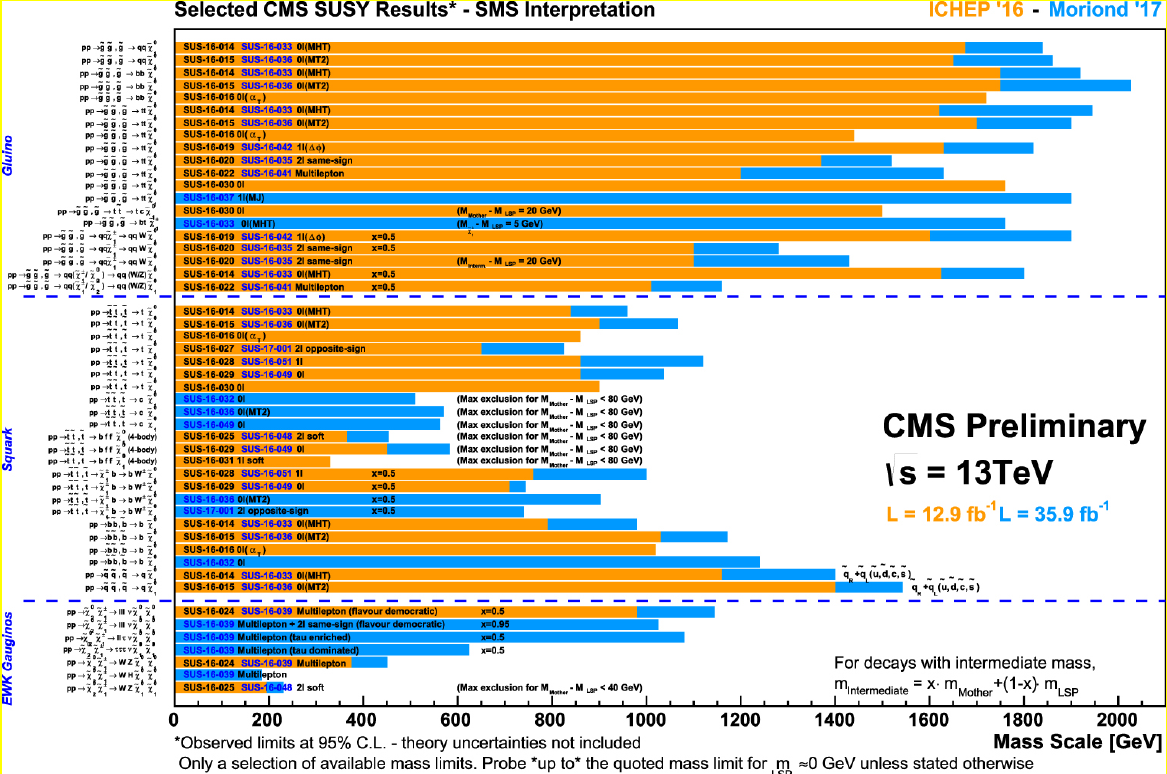
\includegraphics[width=0.4\textwidth]{physics_beyond_the_standard_model/sussy_zoektocht_2017.png}
    }
    \caption{Resultaten van de zoektocht naar SUSY deeltjes}
    \label{fig:physics_beyond_the_standard_model/zoektocht_susy_deeltjes}
\end{figure}

Het grote nadeel aan dit onderzoek is dat er altijd een grote background zal zijn van al de Standaard Model processen die ook gebeuren. In figuren \ref{fig:physics_beyond_the_standard_model/zoektocht_susy_deeltjes} vinden we resultaten voor de zoektocht naar SUSY deeltjes. Hier gaan we niet te diep op in. De massa van het onderzochte deeltje wordt altijd uitgezet tegenover de massa van het lichtste super symmetrie deeltje. In de s-top productie kan je zien dat het grootste gebied al uitgesloten is maar dat er nog kleine gebieden over zijn waar ze zouden kunnen zitten waar veel te grote background processen zijn uit het standaard model.\\
In de samenvatting van deze zoektocht in 2017 kunnen we zien dat voor een groot deel van de faseruimte de supersymmetrie uitgesloten zal zijn maar niet overal.

\subsection{Terug neutrinos}%
\label{sub:terug_neutrinos}

Nog een andere aanwijzing dat het Standaard Model niet helemaal goed zit is de $CP$ schending in de QCD sector. We hebben er niet echt een oplossing voor behalve als we axionen zouden vinden. Kijken we naar de massa van neutrinos tegenover de andere leptonen.

\begin{figure}[h]
    \centering
    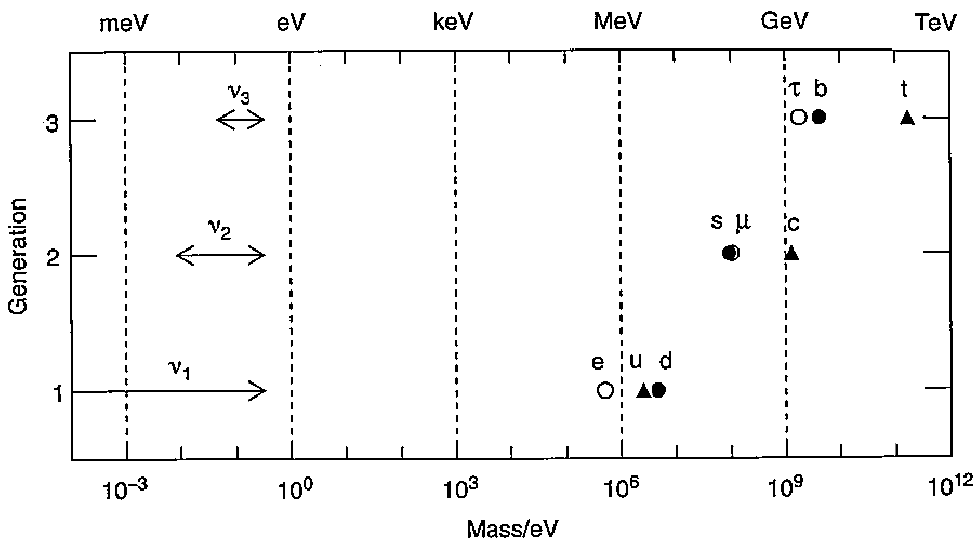
\includegraphics[width=0.5\linewidth]{physics_beyond_the_standard_model/neutrino_massa.png}
    \caption{Massa van neutrinos tegenover de andere leptonen}%
    \label{fig:physics_beyond_the_standard_model/neutrino_massa}
\end{figure}

Wat we zien is dat de massa van de leptonen die in dezelfde generatie zitten altijd dicht bij elkaar liggen behalve voor de neutrinos. Dit geeft naast het feit dat ze alleen linkshandig voorkomen echt wel andere deeltjes zijn dan de gewone leptonen. De massa van de leptonen komt van het Higgs mechanisme. Maar waar komt nu de massa van neutrinos? De massaterm voor fermionen is gegeven door:
\begin{equation}
    \begin{aligned}
        \label{eq:massaterm_fermionen}
        \mathcal{L}_{D}=-m_{f} \bar{f} f=-\frac{g_{f}}{\sqrt{2}} v\left(\bar{f}_{L} f_{R}+\bar{f}_{R} f_{L}\right)
    \end{aligned}
\end{equation}
Deze massaterm voor de fermionen in de Dirac Lagrangiaan is niet verplicht maar blijkbaar is het wel zo. De massa van het fermion is evenredig met de kopppelingconstante aan het Higgs veld en de Higgs vacuum term, $m_f\propto g_f v$. Voor de neutrinos zal deze $g_f$ hoogstens $10^{-12}$ zijn. Belangrijk is dat het steeds een combinatie van links en rechts chirale deeltjes zijn die koppelen aan het Higgs veld. Omdat $\nu_R$ niet interageren in het Standaard Model is het niet mogelijk dat neutrinos te koppelen aan het Higgs veld. Het komt erop neer dat het Standaard model je niet verbied om neutrinos massa te geven maar dit is niet natuurlijk. Een theorie die de neutrinos massa geven is de Majorana theorie die een massaterm geeft aan de neutrinos.
\begin{equation}
    \begin{aligned}
        \label{eq:majorana_massaterm}
        \mathcal{L}_{M}=-\frac{1}{2} M\left(\overline{\nu_{R}^{c}} \nu_{R}+\overline{\nu_{R}} \nu_{R}^{c}\right) \quad \nu^{c}=\hat{C} \hat{P}\nu
    \end{aligned}
\end{equation}
Hierbij zal $\nu_R^c$ overeen komen met een links handig antineutrino. Dit is mogelijk voor nuetrinos maar niet voor bijvoorbeeld elektronen omdat $CP$ van een elektron een positron is. Voegen we de Majorana en Dirac Lagrangiaan samen krijgen we een meer generale massaterm.
\begin{equation}
    \begin{aligned}
        \label{eq:dirac_majorana_massaterm}
        \mathcal{L}_{D M} &=-\frac{1}{2}\left[m_{D} \overline{\nu_{L}} \nu_{R}+m_{D} \overline{\nu_{R}^{c}} \nu_{L}^{c}+M \overline{\nu_{R}^{c}} \nu_{R}\right]+h . c . \\
                          &=-\frac{1}{2}\left(\begin{array}{cc}
                                  \bar{\nu}_{L} & \bar{\nu}_{R}^{c}
                                  \end{array}\right)\left(\begin{array}{cc}
                                  0 & m_{D} \\
                                  m_{D} & M
                                  \end{array}\right)\left(\begin{array}{c}
                                  \nu_{L}^{c} \\
                                  \nu_{R}
                          \end{array}\right)+h . c .
    \end{aligned}
\end{equation}
De eerste 2 termen komen overeen met de termen in de Dirac massaterm maar dan met de aangepaste Majorana neutrino eigentoestanden. Er is ook een extra Majorana term en het hermetisch toegevoegde. Dit kon dan ook herschreven worden in matrix expressies.\\
\begin{minipage}[c]{0.5\textwidth}
    \begin{center}
        \feynmandiagram [vertical=a to b] {
            i1 [particle=\(\nu_R\)]
            -- [anti fermion] a [dot]
            -- [anti fermion] f1 [particle=\(\nu_L\)],
            a -- [scalar] b [particle=\(x\)]
        };
    \end{center}
\end{minipage}\noindent
\begin{minipage}[c]{0.5\textwidth}
    \begin{center}
        \feynmandiagram [horizontal=a to b] {a [particle=\(\nu_R\)] -- [majorana, insertion=0.5, edge label=\(M\)] b [particle=\(\bar{\nu}_L\)]};
    \end{center}
\end{minipage}
Deze 2 massa's moeten hoogst waarschijnlijk verschillend zijn. We hebben bij neutrinos een Dirac en Majorana complonent maar anderzijds hebben we ook massaeigentoestanden. We gaan dus weer een rotatie moeten doen van de ene basis naar de andere. Deze is gegeven in vergelijking \ref{eq:dirac_majorana_massaterm}. Om eigentoestanden van deze matrix te krijgen wat de fysische eigentoestanden zijn moeten we deze diagonaliseren. We krijgen dus een opmenging van de Dirac en Majorana massa tot de massa eigentoestanden.
\begin{equation}
    \begin{aligned}
        \label{eq:dirac_majorana_massa_opmenging}
        m_{\pm}=\frac{M \pm M \sqrt{1+4 m_{D}^{2} / M^{2}}}{2}
    \end{aligned}
\end{equation}
Als we ervan uit gaan dat de Majorana massa veel groter is dan de Dirac massa dan krijgen we enerzijds een licht vooral links handig neutrino $m_{\nu} \approx \frac{m_{D}^{2}}{M}$ of een zwaar vooral rechts handig neutrino met $m_{N} \approx M$. Als we nu verwachten dat de Dirac massa $\approx 1$GeV is en de gewone neutrino massa $m_\nu\approx 0.01$eV dan moet $M\approx 10^{11}$GeV zijn. Dit geeft ons een verklaring waarom we enkel linkshandige neutrinos zien, dit noemen we het Seesaw mechanisme. De voorwaarde is natuurlijk dat we kunnen waarnemen dat het Majorana deeltjes zijn. {\color{green} Dit gedeelte over de massa van de neutrinos is gegeven aan andere slides dan op ufora. Kijk hiervoor naar de opgenomen lessen.}

\subsection{Zoektocht naar BSM fysica}%
\label{sub:zoektocht_naar_bsm_fysica}

Hoe zoeken we nu naar de beyond Standard Model fysica. We kunnen hier direct achter zoeken (bijvoorbeeld zoeken naar SUSY deeltjes). De zoektocht naar donkere materie deeltjes gaat ook nog altijd door (zie figuur \ref{fig:physics_beyond_the_standard_model/donkere_materie_mogelijkheden})

\begin{figure}[h]
    \centering
    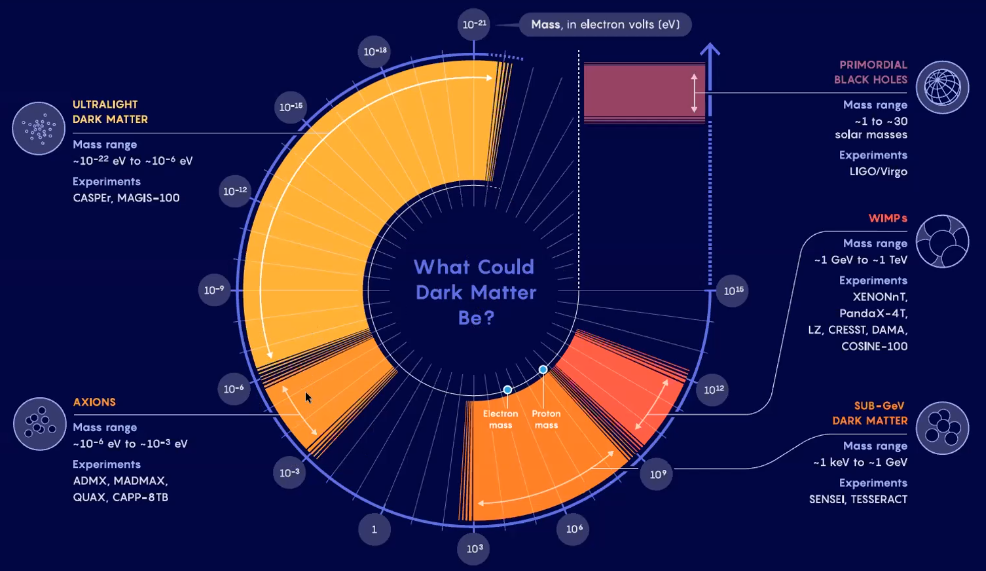
\includegraphics[width=0.5\linewidth]{physics_beyond_the_standard_model/donkere_materie_mogelijkheden.png}
    \caption{Welke deeltjes er donkere materie zouden kunnen zijn}%
    \label{fig:physics_beyond_the_standard_model/donkere_materie_mogelijkheden}
\end{figure}

Het is natuurlijk fantastisch dat we een model hebben dat alle metingen die we tot vandaag de dag hebben gedaan, kan verklaren. Dit is natuurlijk jammer voor het onderzoek naar deze deeltjes. Om te zoeken naar uitzonderingen van het Standaard Model moeten we heel precieze metingen doen van zeldzame vervallen of naar observabelen die eigenlijk verboden zijn in het SM. Het is ook mogelijk om te kijken naar het magnetische moment van het muon $g_2(\mu)$ wat zuiver QED is. Dit is makkelijk uit te rekenen. Het mooie is dat we gevoelig zijn aan alle mogelijke elektrisch geladen deeltjes als we een afwijking zien tussen de berekening voor de gekende deeltjes en de metingen is er een aanleiding dat er nog geladen deeltjes zullen zijn. Het is mogelijk om deze $g_2(\mu)$ met hoge precisie te meten waarbij we vandaag de dag een afwijking van $2.5\sigma$ hebben van de theorie. Dit kan naar de toekomst toe mogelijks bevestiging geven dat er meer geladen deeltjes moeten zijn dan dat we nu kennen.

\subsection{$B_S^0$ verval}%
\label{sub:_b_s_0_verval}

Eén van de bijna niet voorkomende gevallen is het verval van het $B_s^0$ meson. Deze vervalt naar 2 pionen $B_{s}^{0} \rightarrow \mu^{+} \mu^{-}$.

\begin{figure}[h]
    \centering
    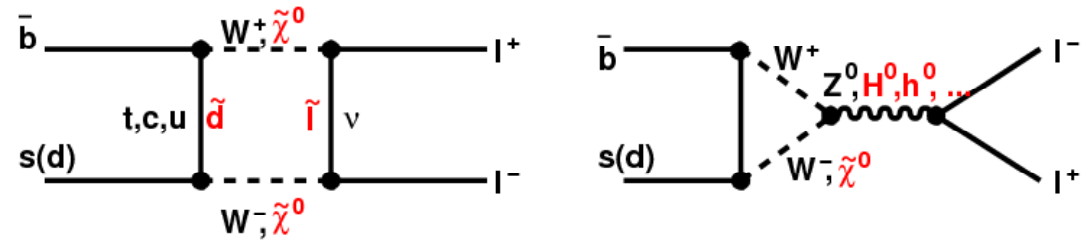
\includegraphics[width=0.7\linewidth]{physics_beyond_the_standard_model/bs_meson_verval.png}
    \caption{Feynman diagrammen van het $B_s^0$ meson verval}%
    \label{fig:physics_beyond_the_standard_model/bs_meson_verval}
\end{figure}

Dit is een 2de orde zwak verval en is dus heel onwaarschijnlijk. Maar 1 in de 300 miljoen $B_s^0$'s zullen vervallen op deze manieren als we kijken naar het Standaard Model. Voegen we aan deze intermediaire deeltjes de SUSY deeltjes toe zouden omdat dit zo onderdrukt wordt in het SM, de SUSY reacties zichtbaar zouden moeten worden. De resultaten van dit onderzoek vindt je in figuur \ref{fig:physics_beyond_the_standard_model/bs_meson_verval_resultaten}.

\begin{figure}[h]
    \centering
    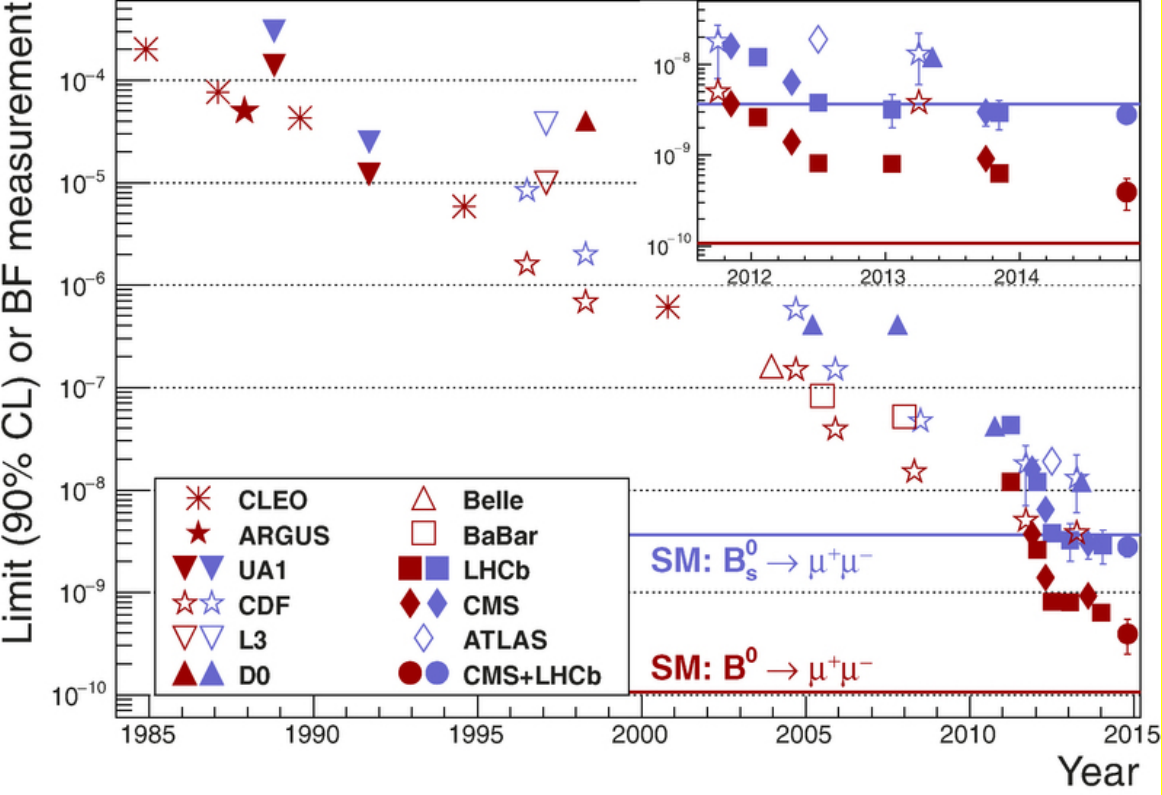
\includegraphics[width=0.6\linewidth]{physics_beyond_the_standard_model/bs_meson_verval_resultaten.png}
    \caption{Resultaten van het $B_s^0$ verval}%
    \label{fig:physics_beyond_the_standard_model/bs_meson_verval_resultaten}
\end{figure}

In 1985 hadden we gemeten dat de branching ratio ten hoogste $10^{-4}$ kon zijn die door de jaren heen verbeteren. Toen het LHC is beginnen draaien was het voor de eerste keer mogelijk om dit verval waar te nemen met een waarschijnlijkheid die overeenkomt met deze van het Standaard Model wat natuurlijk jammer is. We hadden dit liever iets hoger gehad die aanleiding zouden geven tot de SUSY deeltjes. Voor het verval van $\mathbf{B}^{0} \rightarrow \mu^{+} \mu^-$ zijn we nog steeds aan het zoeken wat mogelijks nog een 10tal jaar zal duren.

\begin{figure}[h]
    \centering
    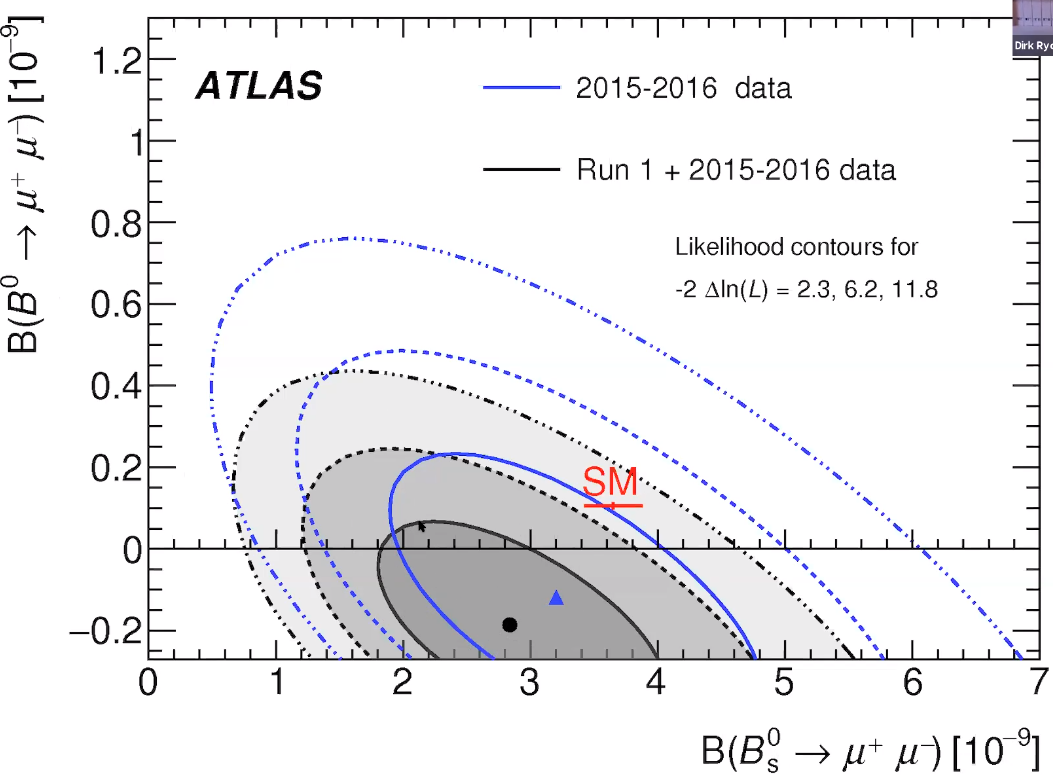
\includegraphics[width=0.6\linewidth]{physics_beyond_the_standard_model/bs_meson_resultaten_vandaag.png}
    \caption{De branching ratios van het $B$ meson verval die we hebben vandaag de dag}%
    \label{fig:physics_beyond_the_standard_model/bs_meson_resultaten_vandaag}
\end{figure}

We zien dat we een lichte afwijking hebben tussen de beste metingen die we vandaag de dag hebben en wat het SM voorspelt. Dit geeft ons aan dat deze heel precieze metingen heel gevoelig zijn voor die modellen voorbij het Standaard Model.\\
Dit voorbeeld van het $B_s^0$ verval is hier gebruikt om aan te tonen dat fysici ook maar mensen zijn. Op cafe is de weddenschap ontstaan dat John Elis in zijn volgende artikel het woord pinguïn moest opnemen. Dit heeft hij weldegelijk gedaan waar hij sprak over het pinguïn diagram waar een $\bar{b}$ met een $s$ vervallen tot een 2 $\bar{s}$ quarks.

\begin{figure}[h]
    \centering
    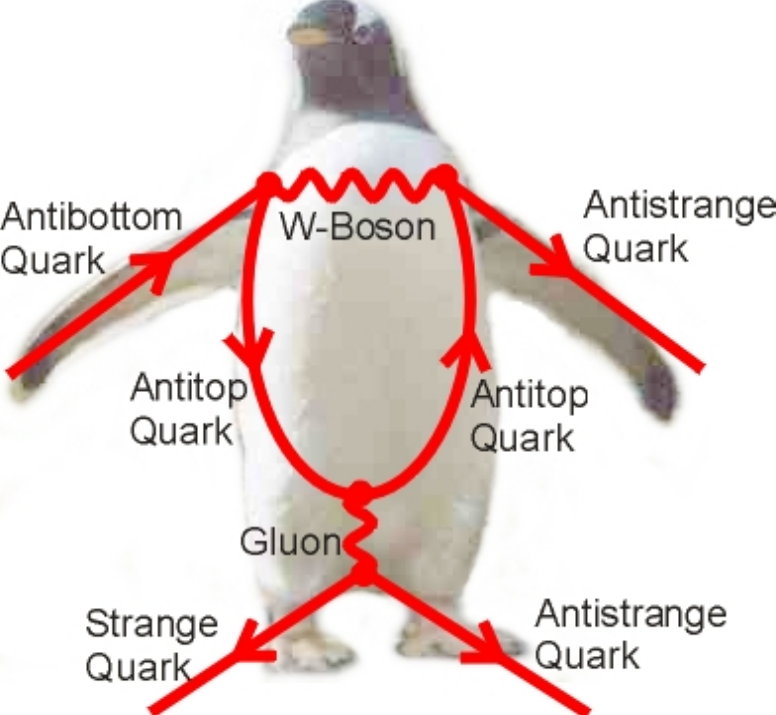
\includegraphics[width=0.8\linewidth]{physics_beyond_the_standard_model/pinguin_diagrammen.png}
    \caption{Pinguïn diagrammen}%
    \label{fig:physics_beyond_the_standard_model/pinguin_diagrammen}
\end{figure}

\end{document}
